\vspace{-0.25em}
\section{Gdev Ecosystem}
\label{sec:ecosystem}
\vspace{-0.25em}

\begin{figure}[t]
 \begin{center}
  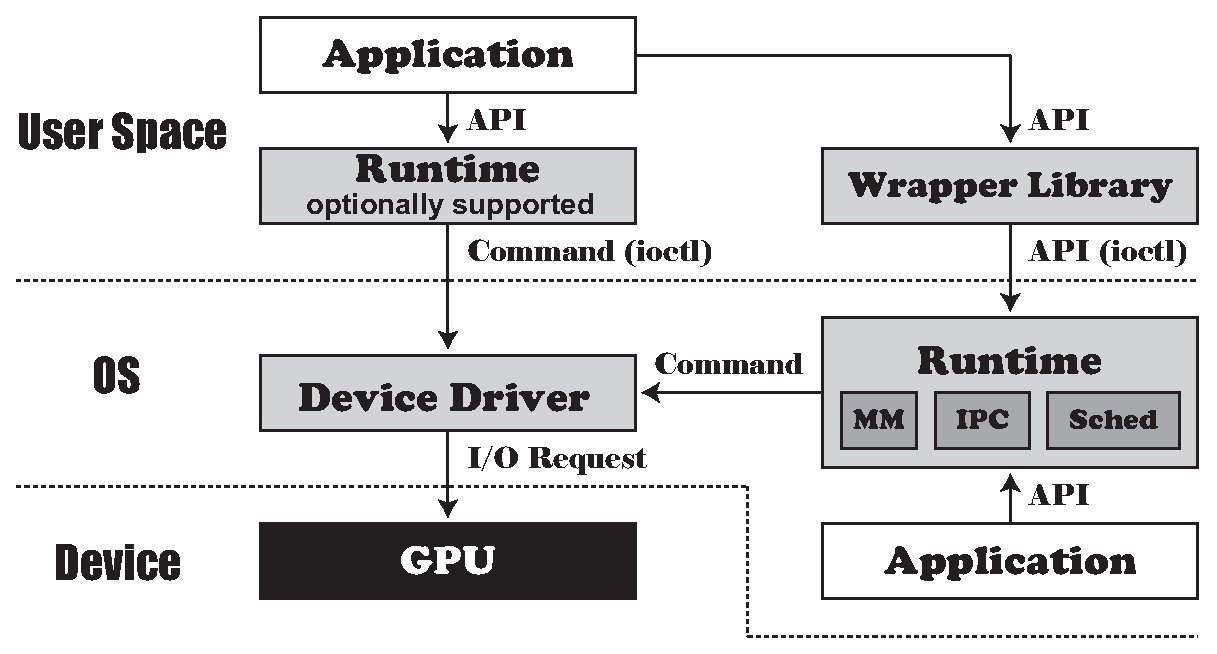
\includegraphics[width=\hsize]{eps/gdev.eps}\\
  \vspace{-0.5em}
  \caption{Logical view of Gdev's ecosystem.}
  \label{fig:gdev}
 \end{center}
 \vspace{-1.5em}
\end{figure}

Gdev aims to enhance GPU resource management, and extend a class
of applications that can use GPUs.
To this end, it integrates the major part of runtime support into the OS.
Figure~\ref{fig:gdev} illustrates the logical view of Gdev's ecosystem.
We still support a traditional execution model where applications make
API calls to the complete user-space runtime library, but this is an
optional path left for compatibility, and the system designer may
disable it to remove the reliability concern discussed in
Section~\ref{sec:introduction}.
In contrast, Gdev's runtime system resides in the OS, which enables both
user-space and OS-space applications to use the same runtime API set
protected by the OS.
Therefore, non-prilileged user-space programs can never bypass the
runtime system with GPU resource management.
There is a wrapper library required for user-space applications, but this is a
tiny piece of software that simply relays API calls to the runtime
system in the OS.

Leveraging this ecosystem, we design an API-driven GPU resource
management scheme.
Figure~\ref{fig:gdev} shows that Gdev allows the OS to manage
API calls, whereas the traditional model translates API calls to GPU
commands before the OS receives them.
As discussed in previous work~\cite{Kato_ATC11}, it is very hard to
analyze GPU commands and recognize the corresponding API calls in the
OS.
Hence, the existing GPU resource management schemes in the
OS~\cite{Bautin_MCNC08, Kato_ATC11} compromise overhead to invoke the
scheduler at every GPU command submission, unless an additional
programming abstraction is provided~\cite{Rossbach_SOSP11}.
On the other hand, Gdev can manage GPU resources along with API calls,
without any additional programming abstractions.

\textbf{Programming Model:}
We provide a set of low-level functions called Gdev API for GPU
programming.
Gdev API can be a useful backend for high-level APIs, such as CUDA,
OpenCL, and HMPP.
The detail of Gdev API can be found at our website~\cite{Gdev}.
Programmers may use either Gdev API directly or a high-level API built
on top of Gdev API.
In this paper, we particularly assume that programmers use ``CUDA Driver
API 4.0''~\cite{CUDA40}.

Gdev uses an existing programming framework and commodity compiler, such
as NVIDIA CUDA Compiler (NVCC)~\cite{CUDA40}.
When a program is compiled, two pieces of binary are generated.
One executes on the CPU, and loads the other binary onto the GPU.
The CPU binary is provided as an executable file or loadable module,
while the GPU binary is an object file.
Hence, both user-space and OS-space applications can use the same
framework: (i) read the GPU binary file and (ii) load it onto the GPU.
The detailed information embedded in the object file, such as code,
static data, stack size, local memory size, and parameter format, may
depend on the programming language, but the framework does not depend on
it once the object file is parsed.

\textbf{Resource Management:}
We provide device memory management and GPU scheduling schemes to manage
GPUs as first-class computing resources.
Specifically, we provide shared device memory for IPC, data swap for
large memory demands, resource-based queuing for throughput, and
bandwidth-aware resource partitioning for virtual GPU isolation.
Since some of these features require access to low-level system
information, such as I/O regions, DMA pages, and task control blocks, it
is not straightfoward for the traditional user-space runtime system to
manage these pieces of information.
Hence, we claim that Gdev is a suitable approach to first-class GPU
resource management.
The concept of Gdev is also not limited to GPUs, but can be
generalized for a broad class of heterogeneous compute devices.

